\section{}
A machine component is modeled as a system comprising a pendulum and a spring, illustrated in 
Fig 1. This setup combines gravitational and spring forces, with the pendulum contributing 
rotational dynamics influenced by gravity, and the spring providing a proportional restoring force. 
The geometric arrangement and interconnection of these components are depicted in Fig 1. 
(Assumption: the rotation is small enough so that the spring only deflects horizontally.)

\begin{figure}[h]
    \centering
    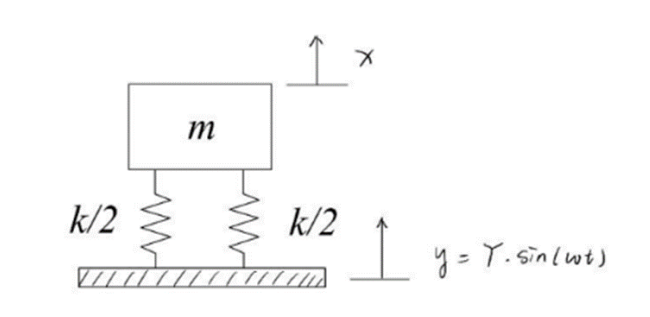
\includegraphics[width=0.5\linewidth]{Questions/Figures/q3 problem diagram.png}
    \caption{The pendulum system connected to a spring}
    \label{fig:q3-png}
\end{figure}
\begin{enumerate}[label=(\alph*)]
    \item (5 pts) Derive the equation of motion for this system using the energy method.
    \item (3 pts) Linearize the equation of motion and derive a formula for the natural frequency of the 
        system.
    \item (2 pts) Compare the natural frequency of this system with the case where there is no spring.
\end{enumerate}

\subsection*{Solution}
\subsection{}
First the total potential energy can be found using the pendulum mass and spring potential energy:
\begin{align*}
    U_{\text{pendulum}} &= m g L (1 - \cos \theta) \\
    U_{\text{spring}} &= \frac{1}{2} k (L \sin \theta)^2  \\
    \implies U_{\text{total}} &= m g L (1 - \cos \theta) + \frac{1}{2} k (L \sin \theta)^2
\end{align*}
Next, the total kinetic energy can be found using the pendulum mass 
\begin{align*}
    T_{\text{pendulum}} &= \frac{1}{2} m \dot{x}^2  = \frac{1}{2} m (L \dot{\theta})^2 
\end{align*}
So total energy is:
\begin{align*}
    E &= T + U \\
    \implies E &= \frac{1}{2} m (L \dot{\theta})^2 + m g L (1 - \cos \theta) + \frac{1}{2} k (L \sin \theta)^2
\end{align*}
Since the system is conservative, the total energy is constant. So,
\begin{align*}
    \frac{dE}{dt} &:= 0 \\
    \frac{dE}{dt} &= m L^2 \dot{\theta} \ddot{\theta} + m g L \sin \theta \dot{\theta} + k L^2 \sin \theta \cos \theta \dot{\theta} 
\end{align*}
\begin{align*}
    \implies \ddot{\theta} + \frac{g}{L} \sin \theta + \frac{k}{m} \sin \theta \cos \theta &= 0 \\
    \Aboxed{\ddot{\theta} + \left(\frac{g}{L} + \frac{k}{m} \cos \theta\right) \sin \theta &= 0}
\end{align*}

\subsection{}
For small angles,
\begin{align*}
    \cos \theta &\approx 1 \\
    \sin \theta &\approx \theta
\end{align*}
So the equation of motion becomes:
\begin{align*}
    \ddot{\theta} + \left(\frac{g}{L} + \frac{k}{m}\right) \theta &= 0
\end{align*}
The natural frequency is given by:
\begin{align*}
    \Aboxed{p = \sqrt{\frac{g}{L} + \frac{k}{m}}}
\end{align*}

\subsection{}
The natural frequency of a normal pendulum is given by:
\begin{align*}
    &p_{\text{pendulum}} = \sqrt{\frac{g}{L}} \\
    &p_{\text{spring \& pendulum}} = \sqrt{\frac{g}{L} + \frac{k}{m}} 
\end{align*}
The spring adds a term $k/m$ to the natural frequency of the system. Since $k/m > 0$,
\begin{align*}
    \Aboxed{\implies p_{\text{spring \& pendulum}} > p_{\text{pendulum}}}
\end{align*}